%% LyX 2.3.6 created this file.  For more info, see http://www.lyx.org/.
%% Do not edit unless you really know what you are doing.
\documentclass[oneside,spanish]{amsart}
\usepackage[T1]{fontenc}
\usepackage[utf8]{inputenc}
\usepackage[a4paper]{geometry}
\geometry{verbose,tmargin=2cm,bmargin=2cm,lmargin=3cm,rmargin=2.5cm}
\usepackage{amsthm}
\usepackage{graphicx}
\usepackage{xargs}[2008/03/08]

\makeatletter

%%%%%%%%%%%%%%%%%%%%%%%%%%%%%% LyX specific LaTeX commands.
%% Because html converters don't know tabularnewline
\providecommand{\tabularnewline}{\\}

%%%%%%%%%%%%%%%%%%%%%%%%%%%%%% Textclass specific LaTeX commands.
\numberwithin{equation}{section}
\numberwithin{figure}{section}
\theoremstyle{plain}
\newtheorem{thm}{\protect\theoremname}
\theoremstyle{remark}
\newtheorem{rem}[thm]{\protect\remarkname}

%%%%%%%%%%%%%%%%%%%%%%%%%%%%%% User specified LaTeX commands.
%% No cambie esta parte a menos que esté seguro de lo que está haciendo.

\usepackage{amsthm}
\usepackage{babel}


\addto\shorthandsspanish{\spanishdeactivate{~<>}}

%%%%%%%%%%%%%%%%%%%%%%%%%%%%%% Textclass specific LaTeX commands.
\numberwithin{equation}{section}
\numberwithin{figure}{section}
\newlength{\lyxlabelwidth} % auxiliary length

\@ifundefined{showcaptionsetup}{}{%
 \PassOptionsToPackage{caption=false}{subfig}}
\usepackage{subfig}
\makeatother

\usepackage{babel}
\addto\shorthandsspanish{\spanishdeactivate{~<>}}

\providecommand{\remarkname}{Observación}
\providecommand{\theoremname}{Teorema}

\begin{document}
\title{Múltiples Registros con los Axiomas de Incidencia de la Geometría
Euclidiana}
\begin{abstract}
Este trabajo explora el concepto de registros en geometría, entendidos
como diferentes formas de representar y comunicar conceptos geométricos.
Estos registros incluyen lingüísticos (uso de lenguaje verbal), gráficos
(dibujos y diagramas), simbólicos (símbolos matemáticos), manipulativos
(uso de materiales físicos) y computacionales (uso de software). Luego,
se destaca la importancia del registro simbólico en la lógica y geometría.

El uso del registro simbólico aporta profundidad al concepto, permitiendo
abstracción y generalización. También ofrece rigor y precisión mediante
el lenguaje formal y las reglas lógicas. La relación con la lógica
es estrecha, ya que el registro simbólico se basa en principios lógicos
y fomenta la comprensión de la lógica y la geometría. La demostración
de un axioma de incidencia se muestra como un ejemplo de cómo el registro
simbólico facilita el razonamiento y la comprensión de los conceptos.

Además, se menciona que la lógica puede abordarse como un juego sintáctico,
lo que la hace más accesible y atractiva para principiantes en matemáticas.
Esta aproximación enfatiza en las reglas y estructura, se relaciona
con el pensamiento abstracto y permite una exploración gradual y experimentación.
\end{abstract}

\maketitle

\section{Introducción}

\subsection{Importancia del trabajo con varios registros}

Entenderemos a los registros en geometría como las diferentes formas
en que se pueden representar y comunicar los conceptos y procesos
geométricos. Los registros son sistemas semióticos que permiten la
expresión y el intercambio de ideas geométricas entre los estudiantes,
los docentes y los materiales de enseñanza. Ver \cite{duval1999semiosis}

Los registros en la geometría pueden incluir:
\begin{itemize}
\item Registros lingüísticos: El uso del lenguaje natural, incluyendo términos,
definiciones, proposiciones y argumentos geométricos expresados en
palabras.
\item Registros gráficos: El uso de dibujos, diagramas, esquemas y representaciones
visuales para ilustrar y comunicar ideas geométricas.
\item Registros simbólicos: El uso de símbolos matemáticos y notación algebraica
para expresar relaciones y propiedades geométricas.
\item Registros manipulativos: El uso de materiales físicos, como modelos
geométricos, construcciones con regla y compás, o manipulación de
objetos tridimensionales, para explorar y experimentar con conceptos
geométricos.
\item Registros computacionales: El uso de software de geometría dinámica,
como Geogebra, para visualizar y manipular objetos geométricos, realizar
construcciones interactivas y realizar cálculos relacionados con la
geometría.
\end{itemize}
El tratamiento de los registros en los axiomas de incidencia de la
geometría euclidiana es importante porque nos permite comprender y
comunicar de manera efectiva los conceptos y propiedades geométricas.
Aquí hay algunas razones clave por las cuales el tratamiento de los
registros es relevante en este contexto:
\begin{itemize}
\item Claridad y comprensión: Los diferentes registros ofrecen diferentes
formas de representar y comprender los axiomas de incidencia. Al utilizar
registros lingüísticos, gráficos, simbólicos y manipulativos, podemos
abordar los axiomas desde múltiples perspectivas, lo que facilita
la comprensión de los conceptos geométricos involucrados.
\item Comunicación efectiva: Los registros nos permiten comunicar los axiomas
de incidencia de la geometría euclidiana de manera clara y precisa.
Cada registro tiene su propio lenguaje y conjunto de convenciones,
lo que permite una comunicación más efectiva entre estudiantes, docentes
y materiales de enseñanza.
\item Representación visual: Los registros gráficos y manipulativos, como
diagramas, modelos físicos y construcciones geométricas, permiten
una representación visual de los axiomas. Esto ayuda a los estudiantes
a visualizar y comprender mejor las relaciones espaciales y las propiedades
geométricas.
\item Abstracción y generalización: El uso de registros simbólicos y lingüísticos,
como fórmulas matemáticas y definiciones formales, permite la abstracción
y generalización de los axiomas de incidencia. Estos registros nos
permiten expresar los axiomas de manera concisa y formal, lo que facilita
su aplicación en diferentes contextos geométricos.
\item Flexibilidad y transferencia: Al trabajar con diferentes registros,
los estudiantes pueden desarrollar habilidades de flexibilidad y transferencia
conceptual. Pueden aprender a traducir y relacionar los conceptos
geométricos entre diferentes registros, lo que les permite aplicar
su conocimiento en una variedad de situaciones geométricas.
\end{itemize}
En este trabajo presentaremos breves comentarios sobre el uso de múltiples
registros para la enseñanza de los axiomas de incidencia de la geometría
euclidiana, pero enfatizando el registro simbólico. 

\section{Requisitos Previos}

Entendimiento básico de la lógica proposicional y el razonamiento
deductivo. Conceptos básicos de Geometría Euclidiana.

\section{Desarrollo}

\subsection{Comentarios sobre el problema teórico}

\newcommandx\pn[1][usedefault, addprefix=\global, 1=]{\mathcal{P}\left(#1\right)}%
 \newcommandx\rc[1][usedefault, addprefix=\global, 1=]{\mathcal{R}\left(#1\right)}%
 \newcommandx\pl[1][usedefault, addprefix=\global, 1=]{\pi\left(#1\right)}%
 \newcommandx\Ir[1][usedefault, addprefix=\global, 1=]{\mathcal{I_{R}}\left(#1\right)}%
 \newcommandx\Ip[1][usedefault, addprefix=\global, 1=]{\mathcal{I_{\pi}}\left(#1\right)}%
 

El conjunto de símbolos propios de la teoría $IGE$ de Incidencia
de la Geometría Euclidiana son $\left\{ =,\pn,\rc,\pl,\Ir,\Ip\right\} $.
Esto quiere decir que debo escribir esta teoría usando solamente estos
símbolos y otros símbolos de la lógica. Por costumbre, a las variables
se las escribe con letras mayúsculas de imprenta, si se quiere hacer
alusión a puntos, con letras minúsculas de imprenta si se quiere hacer
alusión a rectas, y con letras griegas minúsculas si se quiere hacer
alusión a planos. $\pn[A]$ se lee <<$A$ es un punto>>, $\rc[s]$,
<<$s$ es una recta>>, $\pl[\nu]$ <<$\nu$ es un plano>>, $\Ir[P,m]$
<<El punto $P$ está en incidencia con la recta $m$>> o <<$m$
pasa por $P$>> o <<$P$ está en $m$>>, etc; y similarmente para
$\Ip[P,\alpha]$. Para acortar la notación, un pequeño abuso de notación
permitido es $\pn[A,B,C]$ lo entendemos por $\pn[A]\wedge\pn[B]\wedge\pn[C]$
y similarmente para $\rc,\pl$. También escribimos $A,B,C\in r$ en
cuenta de $\Ir[A,r]\wedge\Ir[B,r]\wedge\Ir[C,r]$ y $A,B,C\in\alpha$
en cuenta de $\Ip[A,\alpha]\wedge\Ip[B,\alpha]\wedge\Ip[C,\alpha]$,
siempre que esto no lleve a ambigüedad. Ver \cite{margaris1990first}
\begin{rem}
La pregunta que puede surgir es ¿Cuál es el valor agregado del uso
del registros simbólico? Se puede responder de dos maneras: Primero,
tiene una gramática muy simple (en comparación a los lenguajes naturales
como el inglés o el español). Segundo, es un problema sintáctico,
y por lo tanto, los pasos en una deducción son solamente manipulación
de cadenas.

Para entender mejor el segundo punto en la observación anterior vamos
a considerar lo siguiente: Si en cuenta de leer $\pn[A]$ como <<$A$
es un punto>> se lo leyera como <<$A$ es un jugador de futbol>>,
$\rc[s]$ como <<$s$ es una recta>> se lo leyera como <<$s$ es
un equipo de futbol>> , $\pl[\nu]$ como <<$\nu$ es un plano>>
se lo leyera como , $\Ir[P,m]$ <<El punto $P$ está en incidencia
con la recta $m$>> o <<$m$ pasa por $P$>> o <<$P$ está en
$m$>>, etc; y similarmente para $\Ip[P,\alpha]$.
\end{rem}


\subsection{Ejemplo ilustrativo}

Consideremos el primer axioma de incidencia según la formulación de
\cite{efimov1984geometria}: <<Cualesquiera que sea el punto $A$
y cualesquiera que sea el punto $B$, existe una recta $a$ que pasa
por $A$ y por $B$>>. 
\begin{itemize}
\item Registro lingüístico: Podemos expresar el axioma utilizando lenguaje
verbal, por ejemplo: <<Cualesquiera que sea el punto $A$ y cualesquiera
que sea el punto $B$, existe una recta $a$ que pasa por $A$ y por
$B$>>.
\item Registro gráfico: Podemos representar el axioma mediante un diagrama
que muestra dos puntos $A$ y $B$ y una línea que los conecta. Ver
figura \ref{fig:Axioma-I-de inciden}
\begin{figure}
\begin{centering}
\subfloat[]{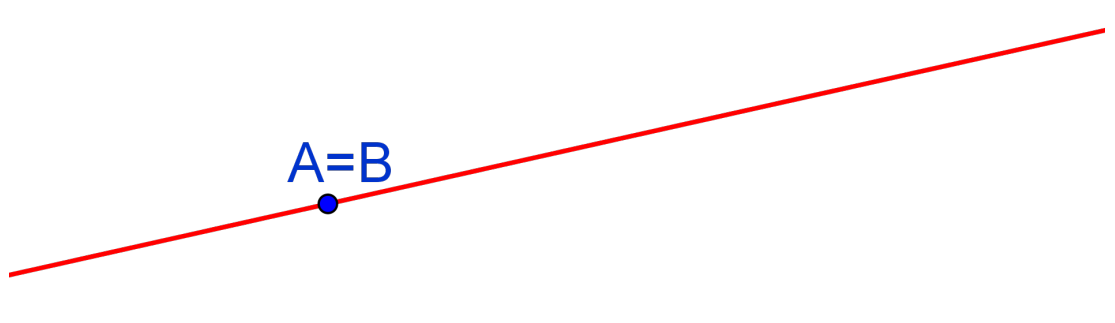
\includegraphics[scale=0.15]{../../LIBRO/Ax1a}

}\subfloat[]{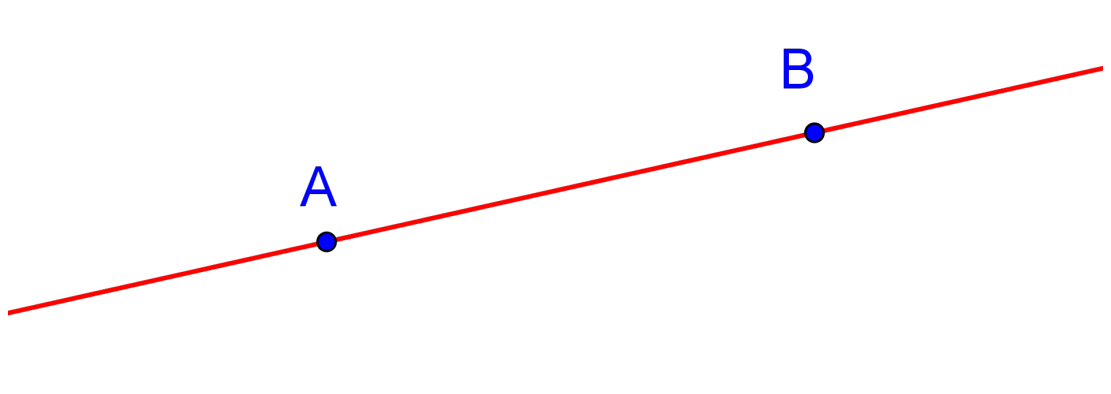
\includegraphics[scale=0.15]{../../LIBRO/Ax1b2b}}
\par\end{centering}
\caption{\label{fig:Axioma-I-de inciden}Axioma 1 de incidencia}
\end{figure}
\item Registro simbólico: Podemos usar símbolos matemáticos para expresar
el axioma, por ejemplo: $\forall A\forall B\exists r\left(\pn[A,B]\rightarrow\rc[r]\wedge A,B\in r\right)$
\item Registro manipulativo: Podemos utilizar regla y compás para construir
físicamente una línea que pase por los puntos $A$ y $B$.
\item Registros computacionales: Con el uso de Geogebra, se puede realizar
dibujos dinámicos, es decir que en este caso pudiera cambiarse las
posiciones relativas de $A$ y de $B$ y ver el cambio de la línea
que pasa por $A$ y por $B$. Para más ejemplos de este recurso puede
verse \cite{geometria11congeogebra}
\end{itemize}
Es común interpretar de la representación lingüística de este axioma
que los puntos $A$ y $B$ son distintos. En esta formulación de los
axiomas de incidencia, no se especifica explícitamente que los puntos
$A$ y $B$ deben ser distintos y, por lo tanto, permite la posibilidad
de que $A$ y $B$ sean el mismo punto. Sin embargo, en el caso de
la representación simbólica, y con un pequeño auxilio de la lógica,
se despejan las dudas. Por ejemplo, revisando la siguiente demostración
con el uso del registro simbólico queda claro una implicación de este
axioma:
\begin{thm}
Si existe un punto, existe una recta: $\vdash\exists A\pn[A]\rightarrow\exists r\rc[r]$
\end{thm}

\begin{proof}
~

\begin{tabular}{|c|l|c|}
\hline 
1. & ~~$\exists A\pn[A]$ & as\tabularnewline
\hline 
2. & ~~~~$\pn[A]$ & c$A$\tabularnewline
\hline 
3. & ~~~~$\forall A\forall B\exists r\left(\pn[A,B]\rightarrow\rc[r]\wedge A,B\in r\right)$ & ax1\tabularnewline
\hline 
4. & ~~~~$\exists r\left(\pn[A,A]\rightarrow\rc[r]\wedge A,A\in r\right)$ & spec\tabularnewline
\hline 
5. & ~~~~~~$\pn[A,A]\rightarrow\rc[r]\wedge A,A\in r$ & c$r$\tabularnewline
\hline 
6. & ~~~~$\,\,\rc[r]$ & SC 2,5\tabularnewline
\hline 
7. & ~~~~$\,\,\exists r\rc[r]$ & $\exists$\tabularnewline
\hline 
8. & ~~~~$\exists r\rc[r]$ & c5\tabularnewline
\hline 
9. & ~~$\exists r\rc[r]$ & c2\tabularnewline
\hline 
10. & $\exists A\pn[A]\rightarrow\exists r\rc[r]$ & DT 1-9\tabularnewline
\hline 
\end{tabular}
\end{proof}
En esta demostración solamente usamos el axioma propio 1, además de
metateoremas del cálculo de predicados con la igualdad. Una explicación
puede ser la siguiente:
\begin{enumerate}
\item Se supone la existencia de un punto $A$ ($\exists A$) y se afirma
que es un punto $(\pn[A]$.
\item Se introduce la notación \textquotedbl cA\textquotedbl{} para denotar
el uso de la regla $C$ 
\item Se utiliza el primer axioma de incidencia.
\item Se realiza una instancia de cuantificador universal, reemplazando
$B$ por $A$ en el axioma, es decir especializando el axioma.
\item Se utiliza nuevamente la regla C pero esta vez en $r$
\item Se utiliza un silogismo o un teorema del calculo de proposiciones
(SC) para concluir que $r$ es una recta.
\item Se utiliza la introducción del cuantificador existencial para afirmar
que existe una recta $r$ 
\item Se descarga la regla C aplicada a $r$.
\item Se descarga la regla C aplicada a $A$.
\item Se aplica el teorema de la deducción y se concluye.
\end{enumerate}

\subsection{Conclusiones}

El ejemplo anterior nos permitió ilustrar que el uso del registro
simbólico en la demostración aporta profundidad al concepto y acerca
el estudio de la lógica a la geometría de varias maneras:
\begin{itemize}
\item Abstracción y generalización: El registro simbólico permite expresar
las ideas y conceptos de manera abstracta utilizando símbolos matemáticos
y lógicos. En el caso de la demostración, se utilizan símbolos como
$\exists$, $\forall$, $\rightarrow$, $\wedge$ para representar
los cuantificadores existenciales y universales, la implicación lógica
y la conjunción, respectivamente. Esta abstracción nos permite generalizar
los razonamientos y aplicarlos a diferentes situaciones geométricas.
\item Rigor y precisión: El registro simbólico proporciona un lenguaje formal
y preciso para expresar las ideas geométricas. Los símbolos y las
reglas de inferencia utilizadas en la lógica matemática nos permiten
establecer argumentos de manera rigurosa y evitar ambigüedades. En
la demostración, el uso de símbolos como $\pn$ $\rc$ $A$, $B$,
$r$ nos permite representar claramente los conceptos de punto, recta
y pertenencia, y establecer las condiciones necesarias para demostrar
la existencia de una recta que pasa por un punto.
\item Relación con la lógica: El registro simbólico utilizado en la demostración
está estrechamente relacionado con los principios y reglas de la lógica
matemática. La expresión de los axiomas y las inferencias lógicas
utilizadas se basan en la estructura formal de la lógica de predicados.
Esto permite una conexión directa entre la lógica y la geometría,
facilitando el estudio de ambos campos y fomentando la comprensión
de sus fundamentos y métodos de razonamiento.
\end{itemize}
Queda un problema que pudiera parecer inalcanzable desde el punto
de vista didáctico y es el de la lógica. Sin embargo, puede explicarse
la lógica como lo que es: \textbf{Un juego sintáctico.}

Explicar la lógica como un juego sintáctico es una forma accesible
y atractiva de abordar esta disciplina sin requerir conocimientos
previos de matemáticas. Aquí hay algunas razones por las cuales esta
aproximación es efectiva:
\begin{itemize}
\item Enfoque en las reglas y la estructura: Al tratar la lógica como un
juego sintáctico, nos centramos en las reglas y la estructura del
lenguaje formal utilizado en la lógica, en lugar de enfocarnos en
el contenido específico o el significado de las proposiciones. Esto
hace que el enfoque inicial sea más accesible y menos intimidante
para quienes no tienen experiencia en matemáticas.
\item Relación con el pensamiento abstracto: El juego sintáctico en la lógica
implica manipular símbolos y aplicar reglas para generar nuevas cadenas
de símbolos. Esta forma de pensamiento abstracto es más cercana a
cómo pensamos y razonamos naturalmente, lo que facilita la comprensión
de la lógica sin la necesidad de conocimientos matemáticos previos.
\item Exploración gradual: La aproximación del juego sintáctico permite
una exploración gradual de la lógica, comenzando con conceptos y reglas
básicas y avanzando hacia conceptos más complejos a medida que se
adquiere confianza y habilidades. Esta progresión gradual es ideal
para quienes se están iniciando en el estudio de la lógica sin una
base matemática sólida.
\item Experimentación e interacción: Los juegos sintácticos en la lógica
a menudo involucran resolver problemas y proponer soluciones, lo que
fomenta la experimentación y la interacción activa con el material.
Esto puede hacer que el proceso de aprendizaje sea más interesante
y entretenido.
\item Enfoque en el proceso más que en los resultados: Al abordar la lógica
como un juego sintáctico, se enfatiza el proceso de razonamiento y
manipulación de símbolos, en lugar de centrarse en la obtención de
resultados específicos. Esto alienta a los estudiantes a centrarse
en el proceso de pensamiento y en la comprensión de las reglas lógicas,
lo que puede llevar a un aprendizaje más profundo y significativo.
\end{itemize}
En conclusión, si se usan los registros en combinación, en especial
el simbólico obtendremos resultados más efectivos y profundos en la
enseñanza de las matemáticas en general y en particular a la geometría.

\bibliographystyle{apalike}
\bibliography{../../SemIsabel2/thesisExample2}

\end{document}
